\documentclass[preprint, 3p,
authoryear]{elsarticle} %review=doublespace preprint=single 5p=2 column
%%% Begin My package additions %%%%%%%%%%%%%%%%%%%

\usepackage[hyphens]{url}

  \journal{An awesome journal} % Sets Journal name

\usepackage{graphicx}
%%%%%%%%%%%%%%%% end my additions to header

\usepackage[T1]{fontenc}
\usepackage{lmodern}
\usepackage{amssymb,amsmath}
% TODO: Currently lineno needs to be loaded after amsmath because of conflict
% https://github.com/latex-lineno/lineno/issues/5
\usepackage{lineno} % add
\usepackage{ifxetex,ifluatex}
\usepackage{fixltx2e} % provides \textsubscript
% use upquote if available, for straight quotes in verbatim environments
\IfFileExists{upquote.sty}{\usepackage{upquote}}{}
\ifnum 0\ifxetex 1\fi\ifluatex 1\fi=0 % if pdftex
  \usepackage[utf8]{inputenc}
\else % if luatex or xelatex
  \usepackage{fontspec}
  \ifxetex
    \usepackage{xltxtra,xunicode}
  \fi
  \defaultfontfeatures{Mapping=tex-text,Scale=MatchLowercase}
  \newcommand{\euro}{€}
\fi
% use microtype if available
\IfFileExists{microtype.sty}{\usepackage{microtype}}{}
\usepackage[]{natbib}
\bibliographystyle{apalike}

\ifxetex
  \usepackage[setpagesize=false, % page size defined by xetex
              unicode=false, % unicode breaks when used with xetex
              xetex]{hyperref}
\else
  \usepackage[unicode=true]{hyperref}
\fi
\hypersetup{breaklinks=true,
            bookmarks=true,
            pdfauthor={},
            pdftitle={Multiple experiences of the self during adolescence a psychometric network analysis},
            colorlinks=false,
            urlcolor=blue,
            linkcolor=magenta,
            pdfborder={0 0 0}}

\setcounter{secnumdepth}{5}
% Pandoc toggle for numbering sections (defaults to be off)


% tightlist command for lists without linebreak
\providecommand{\tightlist}{%
  \setlength{\itemsep}{0pt}\setlength{\parskip}{0pt}}




\usepackage{xcolor}
\usepackage{lmodern}
\usepackage{soul}
\usepackage{booktabs}
\usepackage{longtable}
\usepackage{array}
\usepackage{multirow}
\usepackage{wrapfig}
\usepackage{float}
\usepackage{colortbl}
\usepackage{pdflscape}
\usepackage{tabu}
\usepackage{threeparttable}
\usepackage{threeparttablex}
\usepackage[normalem]{ulem}
\usepackage{makecell}
\usepackage{xcolor}



\begin{document}


\begin{frontmatter}

  \title{Multiple experiences of the self during adolescence a
psychometric network analysis}
    \author[LNC]{Lisa Raoul%
  %
  }
   \ead{lisa.raoul@univ-amu.fr} 
    \author[INT]{Matteo Neri%
  %
  }
   \ead{aaaa@univ-amu.fr} 
    \author[LNC]{Marie-Hélène Grosbras%
  \corref{cor1}%
  }
   \ead{marie-helene.grosbras@univ-amu.fr} 
      \affiliation[LNC]{Aix Marseille Universite, CNRS, LNC, Laboratoire
de Neurosciences Cognitives, Marseille, France}
    \affiliation[INT]{Aix Marseille Universite, CNRS, INT, Institut de
Neurosciences de la Timone, Marseille, France}
    \cortext[cor1]{Corresponding author}
  
  \begin{abstract}
  This is the abstract.

  It consists of two paragraphs.
  \end{abstract}
    \begin{keyword}
    keyword1 \sep 
    keyword2
  \end{keyword}
  
 \end{frontmatter}

\hypertarget{introduction}{%
\section{Introduction}\label{introduction}}

\newpage

\hypertarget{material-and-methods}{%
\section{Material and methods}\label{material-and-methods}}

\hypertarget{sample-recruitment}{%
\subsection{Sample recruitment}\label{sample-recruitment}}

We conducted a voluntary and anonymous online survey accessible on
limesurvey between May 2021 and May 2023. Participants were informed
that the aim of the study was to better understand ``the links between
body and mind during adolescence'' through a video and an explanatory
text presented in the first page of the questionnaire. We collaborated
with schools and sports clubs in various regions of France, and launched
a campaign through email, social media, and word of mouth, inviting
individuals between the ages of 10 and 23 to participate. Ethical
approval for the study was obtained from the University of Marseille.

\hypertarget{measures}{%
\subsection{Measures}\label{measures}}

The whole survey was composed of general information, scales, and
subscales previously validated, as well as two subscales constructed
based on questions from validated scales (Social Touch and Movement
Seeking). All scales that required answers on a Likert scale were
converted to a 5-point scale to facilitate the completion of the survey.
All questions were forced-choice (except for the Resistance to Peer
Influence questionnaire), but participants had the option to answer ``I
do not wish to answer'' or ``I do not understand the question''. They
were also invited to leave any comments/remarks at the end of the
questionnaire. To gather information about survey distribution, we
collected data on how individuals enrolled in the study and postal
codes. We also assessed dominant hand, native language, grade level in
school, and, for university students, their major. In total,
participants answered 171 items, from which we obtain 33 measures for
analysis.

\hypertarget{general-information}{%
\paragraph{General information}\label{general-information}}

Participants were asked to provide information about \textbf{Sex} and
\textbf{Age} as well as gender, weight and height. \textbf{Body Mass
Index} was calculated from weight/height ratio. Using the information on
sex and gender, we derived a binary variable indicating whether the
participant was \textbf{Cisgender} or not. To assess \textbf{Subjective
Economic Status}, participants were asked to rate the economic status
(income) of their family/environment during their upbringing on a 5
points scale (``Very difficult'', ``Difficult'', ``Neither difficult nor
comfortable'', ``Comfortable'', ``Very comfortable''). Participants were
asked to report the number of \textbf{Chronic pain} conditions they had.

\hypertarget{puberty}{%
\paragraph{Puberty}\label{puberty}}

The Pubertal Development Scale (PDS) \citep{petersen_self-report_1988}
contains 5 items assessing pubertal status, including, for both boys and
girls, the presence of a growth spurt, pubic hair, and skin changes. For
girls, 2 items also assess breast development and menarche and for boys,
facial hair growth and voice change. There is a significant correlation
between PDS and pubertal status estimate thought physical exam
\citep{shirtcliff_pubertal_2009}. Each item ranges from 1 (development
has not yet begun) to 4 (development seems completed). From the mean on
the 5 scores, we obtained a continuous puberty index.

\hypertarget{physical-activity}{%
\paragraph{Physical activity}\label{physical-activity}}

We used Saltin-Grimby Physical Activity Level Scale (SGPA) which is a
four-level questionnaire to assess leisure time physical activity
\citep{grimby_saltin-grimby_2015} and have recently been shown to be
successfully to assess physical activity levels in adolescents
\citep{beldo_criterion_2022}. We used the french version recently used
by\citep{isoard-gautheur_relationships_2023}.

\hypertarget{private-and-public-self-consciousness-scale-and-social-anxiety}{%
\paragraph{Private and Public Self Consciousness Scale and Social
Anxiety}\label{private-and-public-self-consciousness-scale-and-social-anxiety}}

We used the 22 items french version \citep{pelletier_lechelle_1990} of
the revised version \citep{scheier_self-consciousness_1985} of the Self
Consciousness Scale (SCS) \citep{fenigstein_public_1975}. The SCS
consists of three subscales. The \textbf{Private Self-Consciousness
subscale} (9 items) allow to assess the extent to which individuals
focus on internal thought, sensations and feelings (e.g.~`'I'm always
trying to figure myself out'`). The \textbf{Public Self-Consciousness
subscale} (7 items) quantify to what extend individual tend to focusing
on oneself as an object of an observer's (e.g.'`I usually worry about
making a good impression'`). The \textbf{Social Anxiety subscale} (6
items), measures distress caused by interacting with others (e.g.'`I
have trouble working when someone is watching me''). 2 Items (6 and 8,
Private Self-Consciousness) were rephrased to be more easily
understandable by younger participants (as there is no validated version
for children nor adolescents in French). 2 Items (16 and 20, Social Self
Consciousness) were modified not to be oriented toward appearance. The
Likert scale range from ``extremely uncharacteristic of me'' (1) to
``extremely characteristic'' (5) with higher values indicating higher
tendency to focus on oneself / be anxious. Internal consistency across
all items in the present study (before imputation for missing data) was
\(\alpha\) = 0.87. (Private SCS \(\alpha\) = 0.78, Public SCS \(\alpha\)
= 0.85, Social Anxiety \(\alpha\) = 0.79)

\hypertarget{perspective-taking-and-empathic-concern}{%
\paragraph{Perspective Taking and Empathic
Concern}\label{perspective-taking-and-empathic-concern}}

We used 2 subscales of the French version \citep{gilet_assessing_2013}
of the Interpersonal Reactivity Index (IRI)
\citep{davis_interpersonal_1980} used on adolescents
\citep{hawk_examining_2013}. \textbf{Perspective Taking} (7 items)
reflected a tendency or ability of the subject to adopt the perspective,
or point of view, of other people (e.g., ``I try to look at everybody's
side of a disagreement before I make a decision'') and is considered as
a measure of cognitive empathy. \textbf{Empathic Concern} (7 items)
concern the tendency to experience feelings of warmth, compassion and
concern for others undergoing negative experiences (e.g., ``When I see
someone being taken advantage of, I feel kind of protective towards
them.'') and is considered as a measure of Affective Empathy. The Likert
scale range from ``this doesn't describe me at all'' (1) to ``this
describes me very well'' (5) with higher values showing higher empathy.
Internal consistency across all items in the present study was
\(\alpha\) = 0.79. (Perspective Taking \(\alpha\) = 0.65, Empathic
Concern \(\alpha\) = 0.78)

\hypertarget{affective-behavioral-and-cognitive-engagement-in-social-media}{%
\paragraph{Affective, behavioral and cognitive engagement in Social
Media}\label{affective-behavioral-and-cognitive-engagement-in-social-media}}

We used the 11 itemsSocial Media Engagement Scale For Adolescents
\citep{ni_development_2020}. The questionnaire looks at social media
engagement through three subscales: \textbf{Behavioral engagement} (4
items) (e.g., ``Using social media is my daily habit''),
\textbf{Cognitive engagement} (3 items) (e.g., ``The support and
encouragement of others on social media is very important to me'') and
\textbf{Affective engagement} (4 items) (e.g., ``I feel bored when I
can't use social media''). The Likert scale range from ``strongly
disagree'' (1) to ``strongly agree'' (5). We translate the questionnaire
as no version actually exist in french and found good measure of
Internal consistency in the whole scale (\(\alpha\) = 0.88) and in the 3
subscales (Behavioral \(\alpha\) = 0.9, Cognitive \(\alpha\) = 0.74,
Affective \(\alpha\) = 0.76)

\hypertarget{body-esteem-for-appearence-for-weight-and-attribution}{%
\paragraph{Body-Esteem for Appearence, for Weight and
Attribution}\label{body-esteem-for-appearence-for-weight-and-attribution}}

We used the french version \citep{valls_etude_2011} of the 23 items
Body-Esteem Scale validated for adolescents
(\citet{mendelson_body-esteem_2001}{]}. The questionnaire consist of
three subscales. The \textbf{Appearance} subscale (10 items) asses
general feelings about one's looks (e.g., `'I like what I see when I
look in the mirror'`). The \textbf{Weight satisfaction} (8 tiems)
investigates perceptions of one's own weight and to which extent one
would like to change it (e.g.,'`I am satisfied with my weight'`). The
\textbf{Attribution} subscale (5 items) deals with the participant's
beliefs about how others perceive her looks (e.g.,'`People like my
looks''). The Likert scale range from ``never'' (1) to ``always'' (5)
with higher scores indicating more positive feelings about appearance,
greater weight satisfaction, and positive beliefs on how others perceive
their bodies. Internal consistency across all items in the present study
was \(\alpha\) = 0.92. (Appearance \(\alpha\) = 0.89, Weight \(\alpha\)
= 0.92, Attribution \(\alpha\) = 0.56).

\hypertarget{body-objectificiation}{%
\paragraph{Body Objectificiation}\label{body-objectificiation}}

We used the french version \citep{wollast_how_2019} of the Body
Surveillance subscale (8 items) of the Objectified Body Consciousness
Scale (OBCS)\citep{mckinley_objectified_1996} which examine the degree
to which individual takes an outsider's stance when viewing his/her body
(e.g., ``I am more concerned with what my body can do than how it
looks''). The Likert scale range from ``Strongly Disagree'' (1) to
``Strongly Agree'' (5) with higher scores indicating strong tendency to
body objectification. Internal consistency across all items in the
present study was \(\alpha\) = 0.73.

\hypertarget{family-peers-and-social-media-appearance-related-pressures}{%
\paragraph{Family, peers and social-media appearance-related
pressures}\label{family-peers-and-social-media-appearance-related-pressures}}

We used the french version \citep{rodgers_psychometric_2016} of the 3
subscales focusing in the appearance-related pressures of the
Sociocultural Attitudes Towards Appearance Questionnaire 4 (SATAQ-4)
\citep{schaefer_development_2015}. These 4-items scales assess pressures
originating from \textbf{Family} (4 items) (e.g., ``I feel pressure from
family members to improve my appearance''), \textbf{Peers} (4 items)
(e.g.,``I feel pressure from my peers to look in better shape''), and
\textbf{Social Media} (4 items) (e.g.,``I feel pressure from the media
to look in better shape''). The Likert scale range from ``definitely
dis-agree'' (1) to ``definitely agree'' (5), with higher scores
indicating greater felt pressure. Following some report of
misunderstanding in young sample in pre-test, we modified formulation of
4 items. Internal consistency across all items in the present study was
\(\alpha\) = 0.78. (Family \(\alpha\) = 0.75, Peers \(\alpha\) = 0.62,
Attribution \(\alpha\) = 0.7).

\hypertarget{private-body-consciousness.}{%
\paragraph{Private body
Consciousness.}\label{private-body-consciousness.}}

We used the private body subscale (5 items) of the Body Consciousness
Questinonaire \citep{miller_consciousness_1981} used in adolescents by
\citet{black_gender_2010}. It adress sensitivity in perception of
internal bodily sensations (e.g., ``I am sensitive to internal bodily
tensions'). The Likert scale range from''extremely uncharacteristic of
me'' (1) to ``extremely characteristic of me'' (5), with higher scores
high sensitivity. Internal consistency across all items in the present
study was \(\alpha\) = 0.68.

\hypertarget{body-noticing-not-distracting-not-worrying-litstening-and-trustring-and-emotional-awareness-of-the-body}{%
\paragraph{Body Noticing, not-distracting, not-worrying, litstening and
trustring and emotional awareness of the
body}\label{body-noticing-not-distracting-not-worrying-litstening-and-trustring-and-emotional-awareness-of-the-body}}

We used 6 subscales of the french version of Multidimensional Assessment
of Interoceptive Awareness (MAIA) \citep{mehling_multidimensional_2012}
validated in youth \citep{jones_exploring_2021}. \textbf{Noticing} (4
items) concern the subjective awareness of body sensations (e.g., ``I
notice changes in my breathing, such as whether it speeds up or slows
down''). \textbf{Not-Distracting} (3 items) investigates how often a
person tends not to ignore sensations of pain or discomfort (e.g., ``I
distract myself from sensations of discomfort''). \textbf{Not-Worrying}
(3 items) assess the extent to which a person don't worries about or
catastrophizes sensations of pain or discomfort (e.g., ``I start to
worry that something is wrong if I feel anydiscomfort'').
\textbf{Emotional Awareness} (5 items) deals with the awareness of the
relationship between emotional and bodily states (e.g., ``I notice how
my body changes when I feel happy/joyful'').\textbf{Body Listening} (3
items) assess how often a person actively attends to their bodily
sensations for insight (e.g., ``When I am upset, I take time to explore
howmy body feels''). \textbf{Body Trusting} (3 items) investigates the
extent to which participants experiences their body as a `safe' and
`trustworthy' source of information (e.g., ``I trust my body
sensations''). The Likert scale range from ``Nerver'' (1) to ``Always''
(5), with higher scores indicating greater felt pressure. Internal
consistency across all items in the present study was \(\alpha\) = 0.76.
(Noticing \(\alpha\) = 0.68, Not-Distracting \(\alpha\) = 0.66,
Not-Worrying \(\alpha\) = 0.55, Emotional Awareness \(\alpha\) = 0.79,
Body Listening \(\alpha\) = 0.78, Body Trusting \(\alpha\) = 0.79).

\hypertarget{resistance-to-peer-influence}{%
\paragraph{Resistance To Peer
Influence}\label{resistance-to-peer-influence}}

We used the Resistance To Peer Influence (RPI) Scale
\citep{steinberg_age_2007}. The scale consists of 10 items that presents
the participant with a pairs of statements (i.e.~`'some people\ldots.but
other people.''). After indicating they belong most, participants are
then asked whether the description is ``Really True'' or ``Sort of
True''.Responses are then coded on a 4-point scale, ranging from
``really true'' for one descriptor to ``really true'' for the other
descriptor, and averaged. Higher scores indicate greater resistance to
peer influence. Internal consistency across all items in the present
study was \(\alpha\) = 0.68.

\hypertarget{social-touch}{%
\paragraph{Social Touch}\label{social-touch}}

We used a 8 items questionnaire derived from Social Touch Questionnaire
(5 items) \citep{wilhelm_social_2001} and Dunn Sensory Profil (3
items)\citep{brown_adolescentadult_2002} to evaluates the extent to
which individuals appreciate touching (e.g., ``I would rather avoid
shaking hands'') and being touched (e.g., ``I generally seek physical
contact with others'') in a social context. One item (``I like petting
animals'') was drop as it was significantly not consistent with others
items. The Likert scale range from ``Nearly Never'' (1) to '' Nearly
Always'' (5), with low scores mean strong avoidance of social touch.
Internal consistency across the 7 items in the present study was
\(\alpha\) = 0.73.

\hypertarget{sensitivity-threshold-and-behavior-to-sensory-stimulation}{%
\paragraph{Sensitivity Threshold and Behavior to Sensory
Stimulation}\label{sensitivity-threshold-and-behavior-to-sensory-stimulation}}

We characterize Sensitivity Threshold and Behavior to Sensory
Stimulation using some items from \citet{brown_adolescentadult_2002}`s
Adult and Adolescents Sensory Profile questionnaire. We include 14 items
related to high and low threshold that measure participants' lack of
response or need for more intense stimuli (high threshold) or
participants' tendency to notice of or to be annoyed with sensory
stimuli (Low threshold). Items related to behavioral response to
sensation discriminate individuals who seek sensation (Sensation
Seeking) from those who avoid sensation (Sensation Avoiding). We used 9
items related to sensory processing of Touch, Movement, and Activity
Level (the original version cover also sensory processing of taste/
smell, visual and audition). In the present study, internal consistency
across items related to sensitivity threshold was \(\alpha\) = 0.69 and,
across those related to behavioral response, was \(\alpha\) = 0.45.

\hypertarget{data-analyses}{%
\subsection{Data Analyses}\label{data-analyses}}

We follow here the standards for psychological network analyses proposed
by \citet{burger_reporting_2022} and the recommendation for quality
assessment recommended by \citet{tomei_network_2022} and
\citet{monteleone_systematic_2021}.

\hypertarget{preprocessing}{%
\subsubsection{Preprocessing}\label{preprocessing}}

Data were prepossessed using python and R. On the 815 participants that
completed the survey until the end, we deleted 75 that answer ``I do not
which to answer'' or ``I don't understand the question'' more than 17
times (10\% of the items). Based on visual check of commentary and
pattern response, 4 datasets were also deleted. Following analyses were
thus performed on 736 participants.

\hypertarget{missing-data-for-network-analysis}{%
\paragraph{Missing Data for network
analysis}\label{missing-data-for-network-analysis}}

In the raw items of final sample, 3.79\% of the data was missing. When
missing values was part of a multi-item measure, the measure was
calculated using the mean of the answered items only. Table ?? reports
the percentage of missing data for each item. Regarding the measures
used for network analyses, 1.12\% of the data was missing. 4 measures
had more than one percent of missing values: Physical activity (3.7\%),
number of chronic pain (13.6\%), economic status (2.9\%) and resistance
to peer influence (14.8\%). The first three were mostly related to a
misunderstanding of the question. The resistance to peer influence
missing rate was mostly related to mistakes in the completion procedure
(answering in the two rather than only one subgroups). Little's MCAR
test was statistically significant (X²(864) = 1080.65, p \textless{}
0.001), indicating data was not missing completely at random (MCAR).
Missing data were handled using multivariate imputation by chained
equations also known fully conditional specification, conducted using
the mice package in R \citep{buuren_mice_2011}. (See supplementary
results for Whole sample analysis on data withou imputation).

\hypertarget{measure-selection}{%
\paragraph{Measure selection}\label{measure-selection}}

We check for topological overlap between the different measure with the
goldbricker algorithm with goldbricker function in R package
networktools \citep{jones_networktools_2017}. This recommended procedure
\citep{tomei_network_2022, monteleone_systematic_2021} asses how much
pairs of nodes in a Network have similar connections to other nodes in
order to identify nodes which most likely measure the same underlying
construct (i.e., are colinear) \citep{jones_networktools_2017}. This
condition would influence the network architecture and inflate
centrality metrics of the nodes \citep{mcnally_network_2021}. After
applying goldbricker Private\_Body\_consciousness and
Noticing\_body\_sensations were removed. The Final Network therefore
comprised 32 measures.

\hypertarget{network-analysis}{%
\subsubsection{Network Analysis}\label{network-analysis}}

\hypertarget{network-estimation}{%
\paragraph{Network estimation}\label{network-estimation}}

We estimate network using a partial correlation graphical least absolute
shrinkage and selection operator (GLASSO) estimator using qgraph.

Regularized partial correlation networks (GLASSO networks) estimate
edges (i.e., the partial correlation between two nodes) that are likely
to be spurious as zero, leading to a more parsimonious and theoretically
more accurate network (Epskamp \& Fried, 2018). Correlations between
nodes in GLASSO networks represent unique partial relationships among
symptoms while accounting for all symptoms in the network. The initial
networks were estimated using polychoric correlations. The resulting
network was dense and had several unexpected negative edges. Thus, per
recommendation of Epskamp and Fried (2018), we used Spearman
correlations in our final analysis.

\hypertarget{network-stability-and-accuracy-check}{%
\paragraph{Network stability and accuracy
check}\label{network-stability-and-accuracy-check}}

\hypertarget{network-comparison}{%
\paragraph{Network comparison}\label{network-comparison}}

\hypertarget{results}{%
\section{Results}\label{results}}

\hypertarget{sample-characteristic}{%
\section{Sample Characteristic}\label{sample-characteristic}}

Table 1 displays descriptive data of the whole survey.

Please make sure that your manuscript follows the guidelines in the
Guide for Authors of the relevant journal. It is not necessary to
typeset your manuscript in exactly the same way as an article, unless
you are submitting to a camera-ready copy (CRC) journal.

For detailed instructions regarding the elsevier article class, see
\url{https://www.elsevier.com/authors/policies-and-guidelines/latex-instructions}

\hypertarget{whole-sample-analysis}{%
\subsection{Whole Sample Analysis}\label{whole-sample-analysis}}

\begin{figure}[H]

{\centering 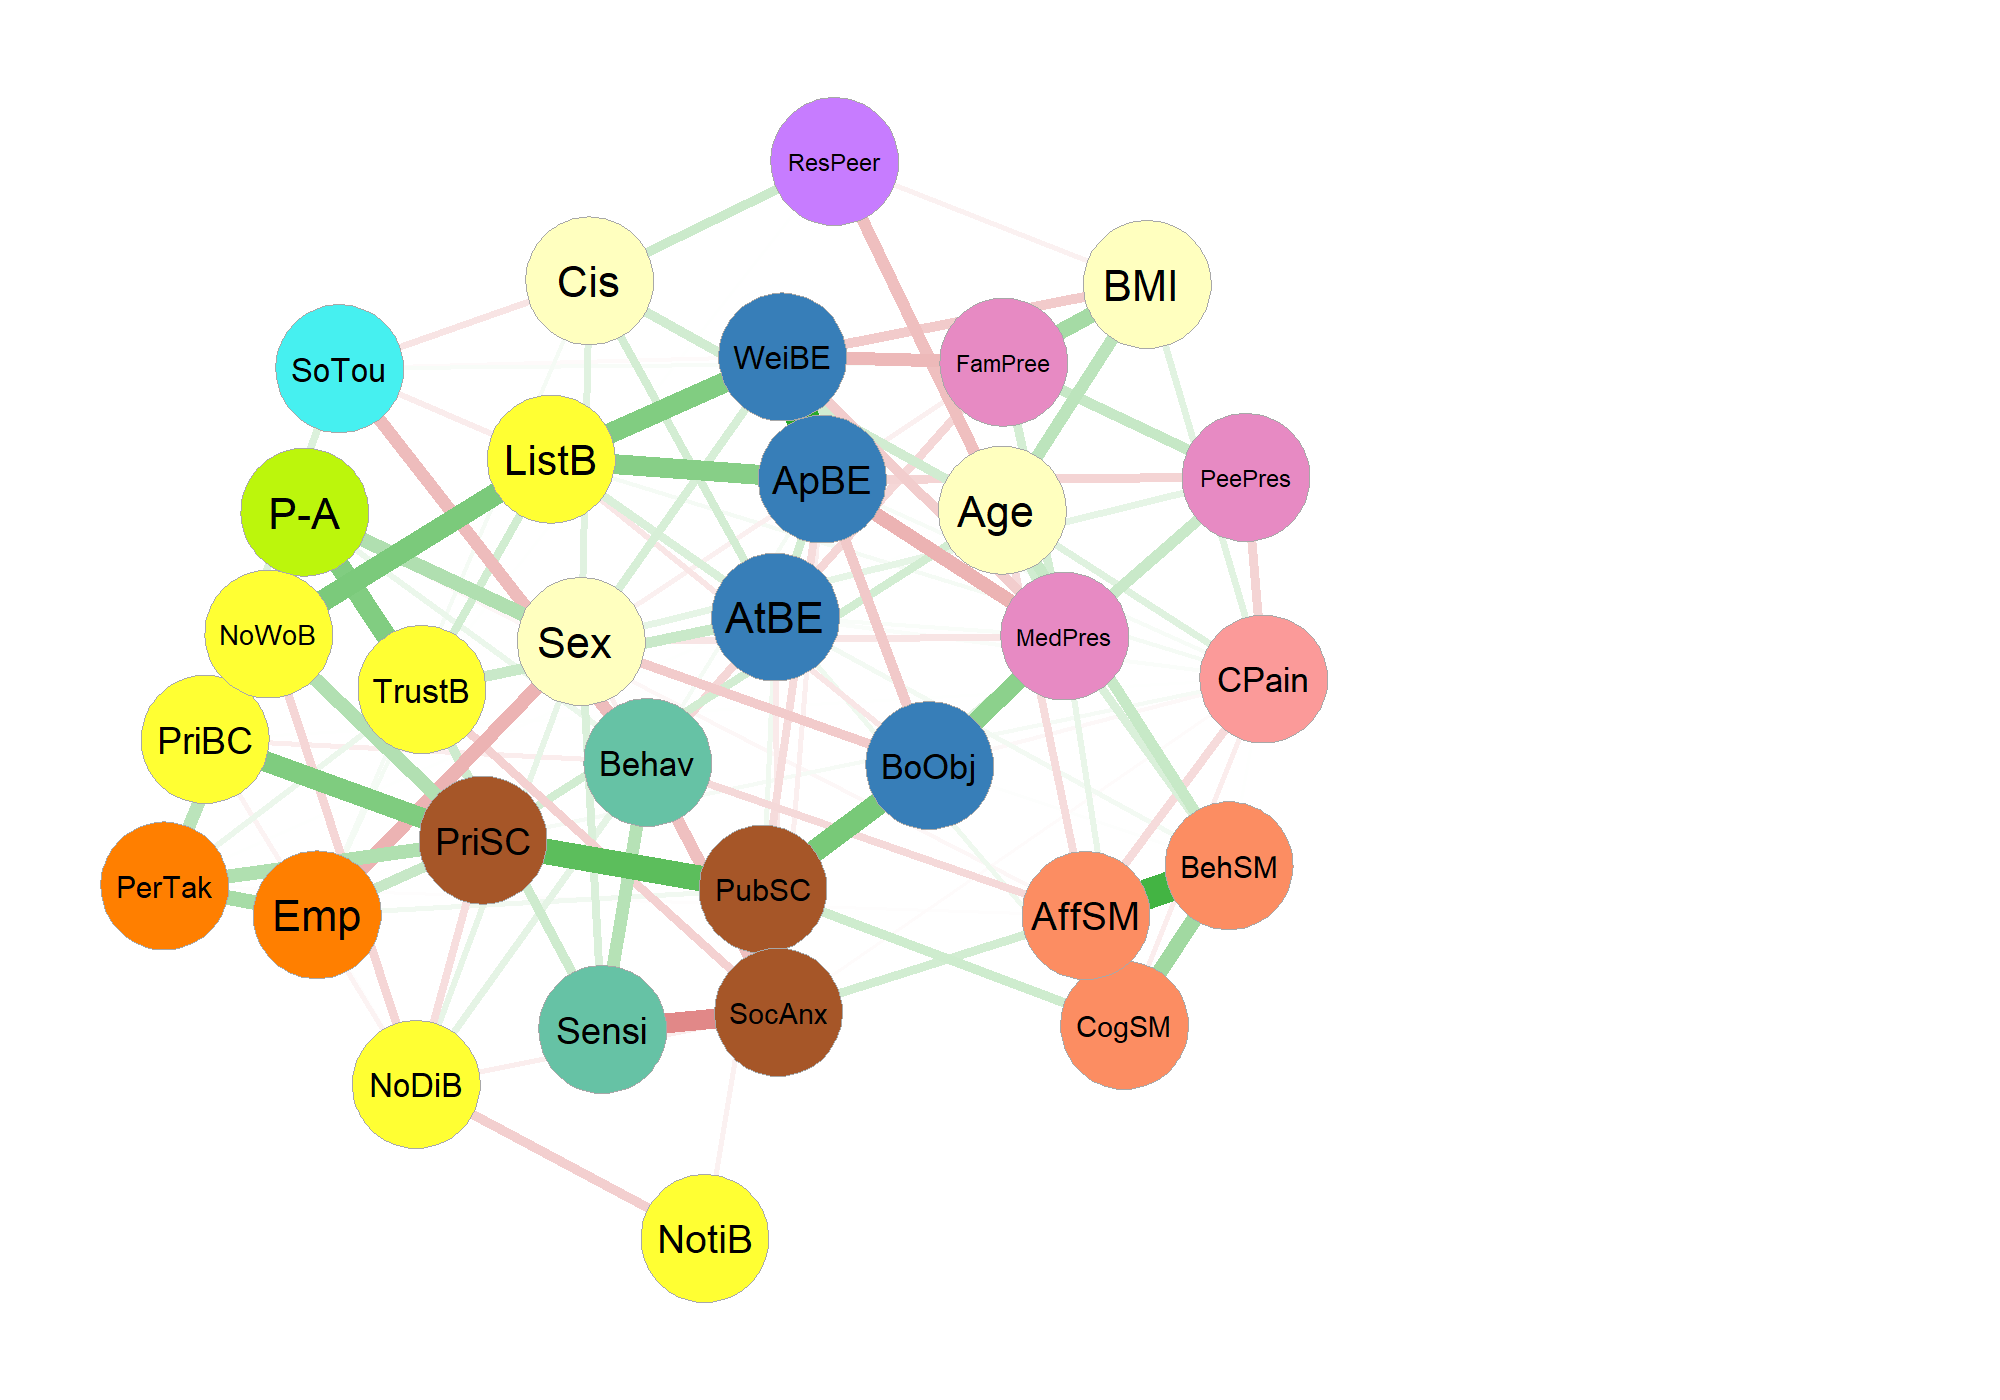
\includegraphics[width=1\linewidth,]{../Figures_Quest/Network_Whole_imputed} 

}

\caption{\label{Whole Sample} Whole Sample Network}\label{fig:unnamed-chunk-3}
\end{figure}

\hypertarget{network-topology-and-centrality}{%
\subsubsection{Network Topology and
Centrality}\label{network-topology-and-centrality}}

\hypertarget{network-stability}{%
\subsubsection{Network Stability}\label{network-stability}}

\hypertarget{group-comparison}{%
\subsection{Group Comparison}\label{group-comparison}}

\hypertarget{discussion}{%
\section{Discussion}\label{discussion}}

rates of onset for several forms of psychopathology peak during
adolescence, \citep{guyer_adolescent_2020}.

\renewcommand\refname{References}
\bibliography{bibthese.bib}


\end{document}
